\documentclass[border=6pt]{standalone}
\usepackage{amsmath}
\usepackage{amssymb}
\usepackage{tikz}
\usetikzlibrary{arrows.meta,calc,decorations.pathreplacing,patterns,shapes.geometric,positioning,shadings,plotmarks}

\begin{document}
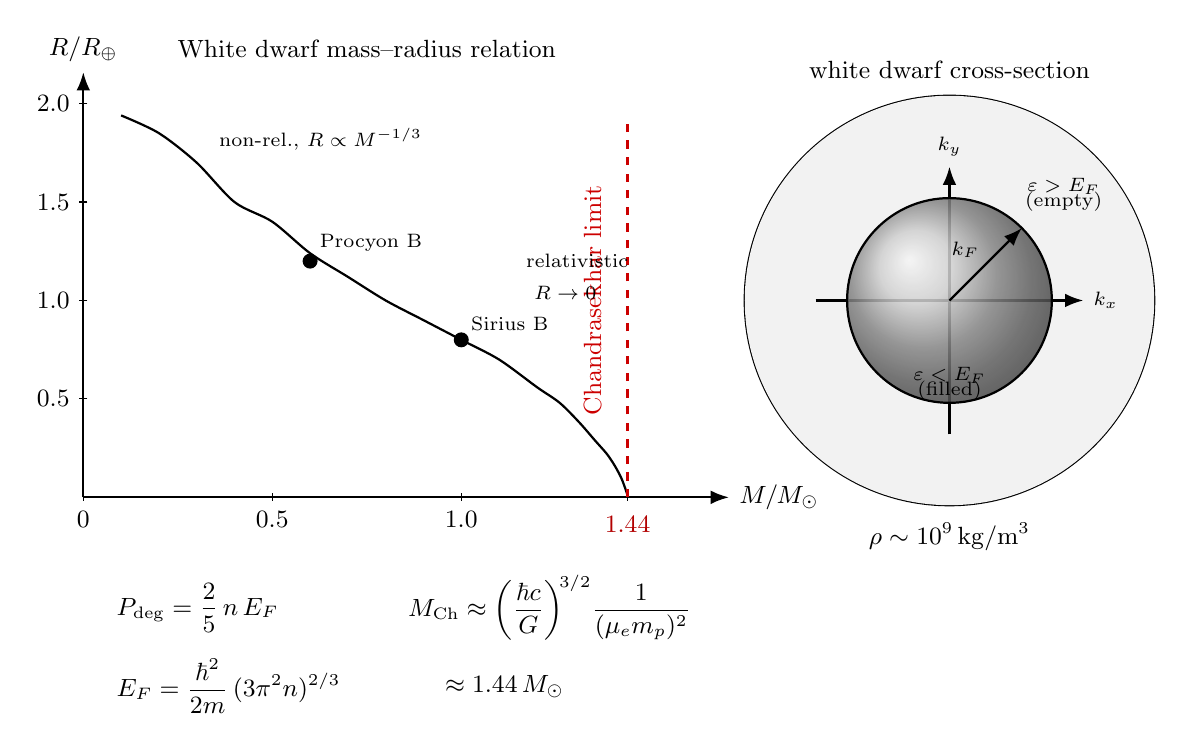
\begin{tikzpicture}[>=Latex]

% =====================================================
% LEFT PANEL: White dwarf mass-radius curve
% =====================================================
\begin{scope}[xshift=0cm]

% Axes
\draw[->,thick] (0,0) -- (8.2,0) node[right] {\small $M / M_\odot$};
\draw[->,thick] (0,0) -- (0,5.4) node[above] {\small $R / R_\oplus$};

% X-axis ticks: 0, 0.5, 1.0, 1.44 (Mch)
\foreach \x/\xv in {0/0, 2.4/0.5, 4.8/1.0} {
    \draw (\x,0.05) -- (\x,-0.05) node[below] {\small $\xv$};
}
\draw (6.912,0.05) -- (6.912,-0.05) node[below=2pt,red!70!black] {\small $1.44$};

% Y-axis ticks
\foreach \y/\yv in {1.25/0.5, 2.5/1.0, 3.75/1.5, 5.0/2.0} {
    \draw (0.05,\y) -- (-0.05,\y) node[left] {\small $\yv$};
}

% Mass-radius curve
% Anchor points: M=0.2->R=1.85, M=0.5->R=1.4, M=0.8->R=1.0, M=1.0->R=0.8, M=1.2->R=0.55, M=1.3->R=0.4, M=1.4->R=0.15, M=1.44->R=0
% Convert: x = M*4.8, y = R*2.5
\draw[thick,black,smooth] plot coordinates {
    (0.48,4.85)
    (0.96,4.625)
    (1.44,4.25)
    (1.92,3.75)
    (2.40,3.50)
    (2.88,3.10)
    (3.36,2.80)
    (3.84,2.50)
    (4.32,2.25)
    (4.80,2.00)
    (5.28,1.75)
    (5.76,1.40)
    (6.05,1.20)
    (6.30,0.95)
    (6.50,0.72)
    (6.65,0.55)
    (6.75,0.40)
    (6.83,0.25)
    (6.88,0.12)
    (6.91,0.03)
};

% Chandrasekhar limit vertical line
\draw[red!80!black,dashed,thick] (6.912,0) -- (6.912,4.8);
\node[red!80!black,rotate=90,anchor=south] at (6.7,2.5) {\small Chandrasekhar limit};

% Observed white dwarfs (data points)
% Sirius B: M=1.0, R=0.8 -> (4.8, 2.0)
\filldraw[black] (4.8,2.0) circle (2.5pt) node[above right] {\scriptsize Sirius B};
% Procyon B: M=0.6, R=1.2 -> (2.88, 3.0)
\filldraw[black] (2.88,3.0) circle (2.5pt) node[above right] {\scriptsize Procyon B};

% Region labels along curve
\node[anchor=west] at (1.6,4.55) {\scriptsize non-rel., $R \propto M^{-1/3}$};
\node[anchor=west] at (5.5,3.0) {\scriptsize relativistic};
\node[anchor=west] at (5.6,2.6) {\scriptsize $R \to 0$};

% Title
\node at (3.6,5.7) {\small White dwarf mass--radius relation};

% Formula annotations (left side, lower)
\node[anchor=west,align=left] at (0.3,-1.4) {\small $P_{\mathrm{deg}} = \dfrac{2}{5}\, n\, E_F$};
\node[anchor=west,align=left] at (0.3,-2.4) {\small $E_F = \dfrac{\hbar^{2}}{2m}\,(3\pi^{2} n)^{2/3}$};
\node[anchor=west,align=left] at (4.0,-1.4) {\small $M_{\mathrm{Ch}} \approx \left(\dfrac{\hbar c}{G}\right)^{\!3/2}\!\dfrac{1}{(\mu_e m_p)^{2}}$};
\node[anchor=west,align=left] at (4.0,-2.4) {\small $\quad\;\, \approx 1.44\, M_\odot$};

\end{scope}

% =====================================================
% RIGHT PANEL: White dwarf cross-section + Fermi sphere
% =====================================================
\begin{scope}[xshift=11cm,yshift=2.5cm]

% Outer dwarf cross-section
\draw[thick] (0,0) circle (2.6cm);
\fill[gray!10] (0,0) circle (2.6cm);

% Density label above
\node[anchor=south] at (0,2.7) {\small white dwarf cross-section};
\node[anchor=north] at (0,-2.7) {\small $\rho \sim 10^{9}\,\mathrm{kg/m^{3}}$};

% Fermi sphere (k-space) inside
% k-axes
\draw[->,thick] (-1.7,0) -- (1.7,0) node[right] {\scriptsize $k_x$};
\draw[->,thick] (0,-1.7) -- (0,1.7) node[above] {\scriptsize $k_y$};

% Filled Fermi sphere (shaded disk)
\shade[ball color=gray!50,opacity=0.85] (0,0) circle (1.3cm);
\draw[thick] (0,0) circle (1.3cm);

% k_F label
\draw[->,thick] (0,0) -- (0.92,0.92) node[midway,above left=-2pt] {\scriptsize $k_F$};

% Annotation: filled vs empty
\node[align=center] at (0,-0.95) {\scriptsize $\varepsilon < E_F$};
\node[align=center] at (0,-1.15) {\scriptsize (filled)};
\node[align=center] at (1.45,1.45) {\scriptsize $\varepsilon > E_F$};
\node[align=center] at (1.45,1.25) {\scriptsize (empty)};

\end{scope}

\end{tikzpicture}
\end{document}
